\documentclass{jsass-ukaren}

\usepackage{float}
\usepackage{graphicx}
\usepackage{siunitx}

\addbibresource{references/example.bib}


\begin{document}

\lectnum{1X01}
\title{第67回宇宙科学技術連合講演会原稿見本}{Sample Format of Paper for the 67th Symposium on Space Science and Technology}

\author{航空一郎}{Ichiro Koku}
\author{宇宙花子}{Hanako Uchu}

\affiliation{日本航空宇宙学会}{JSASS}

\keywords{Space Science, Space Technology, Format Sample}

\begin{abstract}
  This paper instructs how to prepare your manuscript for the 67th Symposium on Space Sciences and Technology.
  All the final manuscripts should be written by word processors with the format specified in this manual.
  You are kindly requested to submit your manuscript in an electronic file on the JSASS website by \textcolor{red}{\textbf{10, August 2023}}.
\end{abstract}

\maketitle


\section{目的および背景}
  これは,第67回宇宙科学技術連合講演会講演集の原稿見本兼作成要領です.
  作成要領は,基本的に日本航空宇宙学会標準の講演会原稿作成要領によりますが,論文原稿の書式に統一性を持たせるために,今回ここに見本として,本作成要領を示します.
  両者に矛盾がある場合は,本稿が優先します.
  できる限り本稿と同じ,もしくは近い書式で作成していただきますようお願いいたします.

\section{書式}\label{sec:sec}
  \cref{tab:fotmat_of_manuscript}に原稿全体の書式を示します.

  \begin{table}[H]
    \centering
    \caption{原稿全体の書式}
    \label{tab:fotmat_of_manuscript}
    \begin{tabular}{|l|l|} \hline
      用紙サイズ & \underline{\textbf{A4版(厳守のこと)}} \\ \hline
      原稿ページ数 & \underline{\textbf{2〜6ページ(厳守のこと)}} \\
      & ページ番号は入れないこと \\ \hline
      余白 & 左右各約\qty{23}{mm}, 上下各約\qty{25}{mm} \\
      & 最低この程度は残して下さい \\ \hline
      字体 & 明朝体 \\
      & (英数字はTimes-New-Roman) \\ \hline
      ファイル形式 & \textcolor{red}{\underline{\textbf{PDFで\qty{5}{MB}以内(厳守のこと)}}} \\ \hline
    \end{tabular}
  \end{table}

\vfil

\section{図および表のフォーマット}
  図は見えにくくならないように,線やシンボルの大きさや説明文の文字の大きさに注意して下さい.
  PDF化で画質が劣化することがありますので,変換後の図から必要な情報が読み取れることを確認して下さい.

  講演集はDVD-ROMで配布しますので,図・表にはカラーも使用可能です.
  キャプションは,図には下,表には上に配置して下さい.
  また,図や表と本文の間には適度な余白を入れて下さい.
  なお、PDFファイル中への動画の埋め込みは,動作環境によっては正常に再生できない可能性があるため,禁止とさせていただきます.

  \begin{figure}[H]
    \centering
    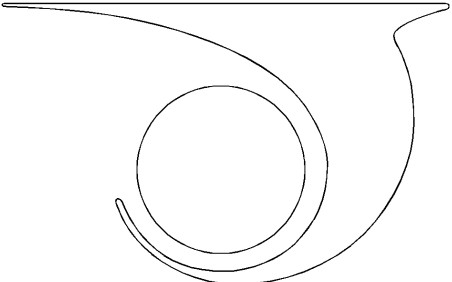
\includegraphics[width=0.75\linewidth]{figures/sample_image.png}
    \caption{図の見本}
    \label{fig:sample_image}
  \end{figure}


\nocite{article_ja_example}
\printbibliography[title=参考文献]

\end{document}